% !TeX spellcheck = pl_PL
%%%%%%%%%%%%%%%%%%%%%%%%%%%%%%%%%%%%%%%%%%%
%                                        %
% Szablon pracy dyplomowej inzynierskiej %
% zgodny  z aktualnymi  przepisami  SZJK %
%                                        %
%%%%%%%%%%%%%%%%%%%%%%%%%%%%%%%%%%%%%%%%%%
%                                        %
%  (c) Krzysztof Simiński, 2018-2023     %
%                                        %
%%%%%%%%%%%%%%%%%%%%%%%%%%%%%%%%%%%%%%%%%%
%                                        %
% Najnowsza wersja szablonów jest        %
% podstępna pod adresem                  %
% github.com/ksiminski/polsl-aei-theses  %
%                                        %
%%%%%%%%%%%%%%%%%%%%%%%%%%%%%%%%%%%%%%%%%%
%
%
% Projekt LaTeXowy zapewnia odpowiednie formatowanie pracy,
% zgodnie z wymaganiami Systemu zapewniania jakości kształcenia.
% Proszę nie zmieniać ustawień formatowania (np. fontu,
% marginesów, wytłuszczeń, kursywy itd. ).
%
% Projekt można kompilować na kilka sposobów.
%
% 1. kompilacja pdfLaTeX
%
% pdflatex main
% bibtex   main
% pdflatex main
% pdflatex main
%
%
% 2. kompilacja XeLaTeX
%
% Kompilatacja przy użyciu XeLaTeXa różni się tym, że na stronie
% tytułowej używany jest font Calibri. Wymaga to jego uprzedniego
% zainstalowania.
%
% xelatex main
% bibtex  main
% xelatex main
% xelatex main
%
%
%%%%%%%%%%%%%%%%%%%%%%%%%%%%%%%%%%%%%%%%%%%%%%%%%%%%%
% W przypadku pytań, uwag, proszę pisać na adres:   %
%      krzysztof.siminski(małpa)polsl.pl            %
%%%%%%%%%%%%%%%%%%%%%%%%%%%%%%%%%%%%%%%%%%%%%%%%%%%%%
%
% Chcemy ulepszać szablony LaTeXowe prac dyplomowych.
% Wypełniając ankietę spod poniższego adresu pomogą
% Państwo nam to zrobić. Ankieta jest całkowicie
% anonimowa. Dziękujemy!


% https://docs.google.com/forms/d/e/1FAIpQLScyllVxNKzKFHfILDfdbwC-jvT8YL0RSTFs-s27UGw9CKn-fQ/viewform?usp=sf_link
%
%%%%%%%%%%%%%%%%%%%%%%%%%%%%%%%%%%%%%%%%%%%%%%%%%%%%%%%%%%%%%%%%%%%%%%%%%

%%%%%%%%%%%%%%%%%%%%%%%%%%%%%%%%%%%%%%%%%%%%%%%
%                                             %
% PERSONALIZACJA PRACY – DANE PRACY           %
%                                             %
%%%%%%%%%%%%%%%%%%%%%%%%%%%%%%%%%%%%%%%%%%%%%%%

% Proszę wpisać swoje dane w poniższych definicjach.

% TODO
% dane autora
\newcommand{\FirstNameAuthor}{Jakub}
\newcommand{\SurnameAuthor}{Kula}
\newcommand{\IdAuthor}{296849}   % numer albumu  (bez $\langle$ i $\rangle$)

% drugi autor:
%\newcommand{\FirstNameCoauthor}{Imię}   % Jeżeli jest drugi autor, to tutaj należy podać imię.
%\newcommand{\SurnameCoauthor}{Nazwisko} % Jeżeli jest drugi autor, to tutaj należy podać nazwisko.
%\newcommand{\IdCoauthor}{$\langle$wpisać właściwy$\rangle$}  % numer albumu drugiego autora (bez $\langle$ i $\rangle$)
% Gdy nie ma drugiego autora, należy zostawić poniższe definicje puste, jak poniżej. Gdy jest drugi autor, należy zakomentować te linie.
\newcommand{\FirstNameCoauthor}{} % Jeżeli praca ma tylko jednego autora, to dane drugiego autora zostają puste.
\newcommand{\SurnameCoauthor}{}   % Jeżeli praca ma tylko jednego autora, to dane drugiego autora zostają puste.
\newcommand{\IdCoauthor}{}  % Jeżeli praca ma tylko jednego autora, to dane drugiego autora zostają puste.
%%%%%%%%%%

\newcommand{\Supervisor}{dr inż. Szymon Ogonowski, prof. PŚ}     % dane promotora (bez $\langle$ i $\rangle$)
\newcommand{\Title}{Tytuł pracy dyplomowej inżynierskiej}           % tytuł pracy po polsku
\newcommand{\TitleAlt}{Thesis title in English}                     % thesis title in English
\newcommand{\Program}{Automatyka i Robotyka}            % kierunek studiów  (bez $\langle$ i $\rangle$)
\newcommand{\Specialisation}{Technologie Informacyjne}     % specjalność  (bez $\langle$ i $\rangle$)
\newcommand{\Departament}{Katedry Pomiarów i Systemów Sterowania}        % katedra promotora  (bez $\langle$ i $\rangle$)

% Jeżeli został wyznaczony promotor pomocniczy lub opiekun, proszę go/ją wpisać ...
\newcommand{\Consultant}{} % dane promotora pomocniczego, opiekuna (bez $\langle$ i $\rangle$)
% ... w przeciwnym razie proszę zostawić puste miejsce jak poniżej:
%\newcommand{\Consultant}{} % brak promotowa pomocniczego / opiekuna

% koniec fragmentu do modyfikacji
%%%%%%%%%%%%%%%%%%%%%%%%%%%%%%%%%%%%%%%%%%


%%%%%%%%%%%%%%%%%%%%%%%%%%%%%%%%%%%%%%%%%%%%%%%
%                                             %
% KONIEC PERSONALIZACJI PRACY                 %
%                                             %
%%%%%%%%%%%%%%%%%%%%%%%%%%%%%%%%%%%%%%%%%%%%%%%

%%%%%%%%%%%%%%%%%%%%%%%%%%%%%%%%%%%%%%%%


%%%%%%%%%%%%%%%%%%%%%%%%%%%%%%%%%%%%%%%%%%%%%%%
%                                             %
% PROSZĘ NIE MODYFIKOWAĆ PONIŻSZYCH USTAWIEŃ! %
%                                             %
%%%%%%%%%%%%%%%%%%%%%%%%%%%%%%%%%%%%%%%%%%%%%%%



\documentclass[a4paper,twoside,12pt]{book}
\usepackage[utf8]{inputenc}                                      
\usepackage[T1]{fontenc}  
\usepackage{amsmath,amsfonts,amssymb,amsthm}
\usepackage[british,polish]{babel} 
\usepackage{indentfirst}
\usepackage{xurl}
\usepackage{xstring}
\usepackage{ifthen}

\usepackage{multirow}


\usepackage{ifxetex}

\ifxetex
	\usepackage{fontspec}
	\defaultfontfeatures{Mapping=tex—text} % to support TeX conventions like ``——-''
	\usepackage{xunicode} % Unicode support for LaTeX character names (accents, European chars, etc)
	\usepackage{xltxtra} % Extra customizations for XeLaTeX
\else
	\usepackage{lmodern}
\fi



\usepackage[margin=2.5cm]{geometry}
\usepackage{graphicx} 
\usepackage{hyperref}
\usepackage{booktabs}
\usepackage{tikz}
\usepackage{pgfplots}
\usepackage{mathtools}
\usepackage{geometry}
\usepackage{subcaption}   % subfigures
\usepackage[page]{appendix} % toc,
\renewcommand{\appendixtocname}{Dodatki}
\renewcommand{\appendixpagename}{Dodatki}
\renewcommand{\appendixname}{Dodatek}

\usepackage{csquotes}
\usepackage[natbib=true,backend=bibtex,maxbibnames=99]{biblatex}  % kompilacja bibliografii BibTeXem
%\usepackage[natbib=true,backend=biber,maxbibnames=99]{biblatex}  % kompilacja bibliografii Biberem
\bibliography{biblio}

\usepackage{ifmtarg}   % empty commands  

\usepackage{setspace}
\onehalfspacing


\frenchspacing



%%%% TODO LIST GENERATOR %%%%%%%%%

\usepackage{color}
\definecolor{brickred}      {cmyk}{0   , 0.89, 0.94, 0.28}

\makeatletter \newcommand \kslistofremarks{\section*{Uwagi} \@starttoc{rks}}
  \newcommand\l@uwagas[2]
    {\par\noindent \textbf{#2:} %\parbox{10cm}
{#1}\par} \makeatother


\newcommand{\ksremark}[1]{%
{%\marginpar{\textdbend}
{\color{brickred}{[#1]}}}%
\addcontentsline{rks}{uwagas}{\protect{#1}}%
}

\newcommand{\comma}{\ksremark{przecinek}}
\newcommand{\nocomma}{\ksremark{bez przecinka}}
\newcommand{\styl}{\ksremark{styl}}
\newcommand{\ortografia}{\ksremark{ortografia}}
\newcommand{\fleksja}{\ksremark{fleksja}}
\newcommand{\pauza}{\ksremark{pauza `--', nie dywiz `-'}}
\newcommand{\kolokwializm}{\ksremark{kolokwializm}}
\newcommand{\cudzyslowy}{\ksremark{,,polskie cudzysłowy''}}

%%%%%%%%%%%%%% END OF TODO LIST GENERATOR %%%%%%%%%%%

\newcommand{\printCoauthor}{%		
    \StrLen{\FirstNameCoauthor}[\FNCoALen]
    \ifthenelse{\FNCoALen > 0}%
    {%
		{\large\bfseries\Coauthor\par}
	
		{\normalsize\bfseries \LeftId: \IdCoauthor\par}
    }%
    {}
} 

%%%%%%%%%%%%%%%%%%%%%
\newcommand{\autor}{%		
    \StrLen{\FirstNameCoauthor}[\FNCoALenXX]
    \ifthenelse{\FNCoALenXX > 0}%
    {\FirstNameAuthor\ \SurnameAuthor, \FirstNameCoauthor\ \SurnameCoauthor}%
	{\FirstNameAuthor\ \SurnameAuthor}%
}
%%%%%%%%%%%%%%%%%%%%%

\StrLen{\FirstNameCoauthor}[\FNCoALen]
\ifthenelse{\FNCoALen > 0}%
{%
\author{\FirstNameAuthor\ \SurnameAuthor, \FirstNameCoauthor\ \SurnameCoauthor}
}%
{%
\author{\FirstNameAuthor\ \SurnameAuthor}
}%

%%%%%%%%%%%% ZYWA PAGINA %%%%%%%%%%%%%%%
% brak kapitalizacji zywej paginy
\usepackage{fancyhdr}
\pagestyle{fancy}
\fancyhf{}
\fancyhead[LO]{\nouppercase{\it\rightmark}}
\fancyhead[RE]{\nouppercase{\it\leftmark}}
\fancyhead[LE,RO]{\it\thepage}


\fancypagestyle{tylkoNumeryStron}{%
   \fancyhf{} 
   \fancyhead[LE,RO]{\it\thepage}
}

\fancypagestyle{bezNumeracji}{%
   \fancyhf{} 
   \fancyhead[LE,RO]{}
}


\fancypagestyle{NumeryStronNazwyRozdzialow}{%
   \fancyhf{} 
   \fancyhead[LE]{\nouppercase{\autor}}
   \fancyhead[RO]{\nouppercase{\leftmark}} 
   \fancyfoot[CE, CO]{\thepage}
}


%%%%%%%%%%%%% OBCE WTRETY  
\newcommand{\obcy}[1]{\emph{#1}}
\newcommand{\english}[1]{{\selectlanguage{british}\obcy{#1}}}
%%%%%%%%%%%%%%%%%%%%%%%%%%%%%

% polskie oznaczenia funkcji matematycznych
\renewcommand{\tan}{\operatorname {tg}}
\renewcommand{\log}{\operatorname {lg}}

% jeszcze jakies drobiazgi

\newcounter{stronyPozaNumeracja}

%%%%%%%%%%%%%%%%%%%%%%%%%%% 
\newcommand{\printOpiekun}[1]{%		

    \StrLen{\Consultant}[\mystringlen]
    \ifthenelse{\mystringlen > 0}%
    {%
       {\large{\bfseries OPIEKUN, PROMOTOR POMOCNICZY}\par}
       
       {\large{\bfseries \Consultant}\par}
    }%
    {}
} 
%
%%%%%%%%%%%%%%%%%%%%%%%%%%%%%%%%%%%%%%%%%%%%%%
 
% Proszę nie modyfikować poniższych definicji!
\newcommand{\Author}{\FirstNameAuthor\ \MakeUppercase{\SurnameAuthor}} 
\newcommand{\Coauthor}{\FirstNameCoauthor\ \MakeUppercase{\SurnameCoauthor}}
\newcommand{\Type}{PROJEKT INŻYNIERSKI}
\newcommand{\Faculty}{Wydział Automatyki, Elektroniki i Informatyki} 
\newcommand{\Polsl}{Politechnika Śląska}
\newcommand{\Logo}{politechnika_sl_logo_bw_pion_pl.pdf}
\newcommand{\LeftId}{Nr albumu}
\newcommand{\LeftProgram}{Kierunek}
\newcommand{\LeftSpecialisation}{Specjalność}
\newcommand{\LeftSUPERVISOR}{PROWADZĄCY PRACĘ}
\newcommand{\LeftDEPARTMENT}{KATEDRA}
%%%%%%%%%%%%%%%%%%%%%%%%%%%%%%%%%%%%%%%%%%%%%%

%%%%%%%%%%%%%%%%%%%%%%%%%%%%%%%%%%%%%%%%%%%%%%%
%                                             %
% KONIEC USTAWIEŃ                             %
%                                             %
%%%%%%%%%%%%%%%%%%%%%%%%%%%%%%%%%%%%%%%%%%%%%%%




%%%%%%%%%%%%%%%%%%%%%%%%%%%%%%%%%%%%%%%%%%%%%%%
%                                             %
% MOJE PAKIETY, USTAWIENIA ITD                %
%                                             %
%%%%%%%%%%%%%%%%%%%%%%%%%%%%%%%%%%%%%%%%%%%%%%%

% Tutaj proszę umieszczać swoje pakiety, makra, ustawienia itd.


 
%%%%%%%%%%%%%%%%%%%%%%%%%%%%%%%%%%%%%%%%%%%%%%%%%%%%%%%%%%%%%%%%%%%%%
% listingi i fragmentu kodu źródłowego 
% pakiet: listings lub minted
% % % % % % % % % % % % % % % % % % % % % % % % % % % % % % % % % % % 

% biblioteka listings
\usepackage{listings}
\lstset{%
morekeywords={string,exception,std,vector},% słowa kluczowe rozpoznawane przez pakiet listings
language=C++,% C, Matlab, Python, SQL, TeX, XML, bash, ... – vide https://www.ctan.org/pkg/listings
commentstyle=\textit,%
identifierstyle=\textsf,%
keywordstyle=\sffamily\bfseries, %\texttt, %
%captionpos=b,%
tabsize=3,%
frame=lines,%
numbers=left,%
numberstyle=\tiny,%
numbersep=5pt,%
breaklines=true,%
escapeinside={@*}{*@},%
}

% % % % % % % % % % % % % % % % % % % % % % % % % % % % % % % % % % % 
% pakiet minted
%\usepackage{minted}

% pakiet wymaga specjalnego kompilowania:
% pdflatex -shell-escape main.tex
% xelatex  -shell-escape main.tex

%\usepackage[chapter]{minted} % [section]
%%\usemintedstyle{bw}   % czarno-białe kody 
%
%\setminted % https://ctan.org/pkg/minted
%{
%%fontsize=\normalsize,%\footnotesize,
%%captionpos=b,%
%tabsize=3,%
%frame=lines,%
%framesep=2mm,
%numbers=left,%
%numbersep=5pt,%
%breaklines=true,%
%escapeinside=@@,%
%}

%%%%%%%%%%%%%%%%%%%%%%%%%%%%%%%%%%%%%%%%%%%%%%%%%%%%%%%%%%%%%%%%%%%%%



%%%%%%%%%%%%%%%%%%%%%%%%%%%%%%%%%%%%%%%%%%%%%%%
%                                             %
% KONIEC MOICH USTAWIEŃ                       %
%                                             %
%%%%%%%%%%%%%%%%%%%%%%%%%%%%%%%%%%%%%%%%%%%%%%%



%%%%%%%%%%%%%%%%%%%%%%%%%%%%%%%%%%%%%%%%


\begin{document}
%\kslistofremarks

\frontmatter

%%%%%%%%%%%%%%%%%%%%%%%%%%%%%%%%%%%%%%%%%%%%%%%
%                                             %
% PROSZĘ NIE MODYFIKOWAĆ STRONY TYTUŁOWEJ!    %
%                                             %
%%%%%%%%%%%%%%%%%%%%%%%%%%%%%%%%%%%%%%%%%%%%%%%


%%%%%%%%%%%%%%%%%%  STRONA TYTUŁOWA %%%%%%%%%%%%%%%%%%%
\pagestyle{empty}
{
	\newgeometry{top=1.5cm,%
		bottom=2.5cm,%
		left=3cm,
		right=2.5cm}

	\ifxetex
		\begingroup
		\setsansfont{Calibri}

	\fi
	\sffamily
	\begin{center}
		\includegraphics[width=50mm]{\Logo}


		{\Large\bfseries\Type\par}

		\vfill  \vfill

		{\large\Title\par}

		\vfill

		{\large\bfseries\Author\par}

		{\normalsize\bfseries \LeftId: \IdAuthor}

		\printCoauthor

		\vfill

		{\large{\bfseries \LeftProgram:} \Program\par}

		{\large{\bfseries \LeftSpecialisation:} \Specialisation\par}

		\vfill  \vfill 	\vfill 	\vfill 	\vfill 	\vfill 	\vfill

		{\large{\bfseries \LeftSUPERVISOR}\par}

		{\large{\bfseries \Supervisor}\par}

		{\large{\bfseries \LeftDEPARTMENT\ \Departament} \par}

		{\large{\bfseries \Faculty}\par}

		\vfill  \vfill


		\printOpiekun{\Consultant}

		\vfill  \vfill

		{\large\bfseries  Gliwice \the\year}

	\end{center}
	\ifxetex
		\endgroup
	\fi
	\restoregeometry
}

%%%%%%%%%%%%%%%%%%%%%%%%%%%%%%%%%%%%%%%%%%%%%%%
%                                             %
% KONIEC STRONY TYTUŁOWEJ                     %
%                                             %
%%%%%%%%%%%%%%%%%%%%%%%%%%%%%%%%%%%%%%%%%%%%%%%  


\cleardoublepage

\rmfamily\normalfont
\pagestyle{empty}


%%% No to zaczynamy pisać pracę :-) %%%%

% TODO
\subsubsection*{Tytuł pracy}
\Title

\subsubsection*{Streszczenie}
(Streszczenie pracy – odpowiednie pole w systemie APD powinno zawierać kopię tego streszczenia.)

\subsubsection*{Słowa kluczowe}
(2-5 slow (fraz) kluczowych, oddzielonych przecinkami)

\subsubsection*{Thesis title}
\begin{otherlanguage}{british}
	\TitleAlt
\end{otherlanguage}

\subsubsection*{Abstract}
\begin{otherlanguage}{british}
	(Thesis abstract – to be copied into an appropriate field during an electronic submission – in English.)
\end{otherlanguage}
\subsubsection*{Key words}
\begin{otherlanguage}{british}
	(2-5 keywords, separated by commas)
\end{otherlanguage}




%%%%%%%%%%%%%%%%%% SPIS TRESCI %%%%%%%%%%%%%%%%%%%%%%
% Add \thispagestyle{empty} to the toc file (main.toc), because \pagestyle{empty} doesn't work if the TOC has multiple pages
\addtocontents{toc}{\protect\thispagestyle{empty}}
\tableofcontents

%%%%%%%%%%%%%%%%%%%%%%%%%%%%%%%%%%%%%%%%%%%%%%%%%%%%%
\setcounter{stronyPozaNumeracja}{\value{page}}
\mainmatter
\pagestyle{empty}

\cleardoublepage

\pagestyle{NumeryStronNazwyRozdzialow}

%%%%%%%%%%%%%% wlasciwa tresc pracy %%%%%%%%%%%%%%%%%

% TODO
\chapter{Wstęp}
\label{ch:wstep}
\section{Cel i zakre pracy}
wprowadzenie w problem/zagadnienie
\section{Aktualny stan wiedzy}
osadzenie tematu w kontekście aktualnego stanu wiedzy (\english{state of the art}) o poruszanym problemie\\
studia literaturowe \cite{bib:artykul,bib:ksiazka,bib:konferencja,bib:internet} -  opis znanych rozwiązań (także opisanych naukowo, jeżeli problem jest poruszany w publikacjach naukowych), algorytmów,
\section{Charakterystyka rozdziałów}
Krótkie wprowadzenie do zawartości
Zarys głównych punktów i celów rozdziału

\section{Wkład autora}
jednoznaczne określenie wkładu autora, w przypadku prac wieloosobowych – tabela z autorstwem poszczególnych elementów pracy
Wzory
\begin{align}
	y = \frac{\partial x}{\partial t}
\end{align}
jak i pojedyncze symbole $x$ i $y$  składa się w trybie matematycznym.



\chapter{Zastosowane narzędzia w pracy}
\label{ch:wymagania-i-narzedzia}
% Opis narzędzi które były uzywane podczas programowania, Wiekszy opis pythona i tensorflow, ich "specyfikacja" plusy i minusy, jakie były inne mozliwe wybory oraz czemu zostały wybrane akurat te rozwiązania, krótszy opis pozostałych biblotek uzytych podczas programownia takich jak numpy, plotlib czy pandas
\section{Python}
Wybór głónego języka progarmowania zastowanego w projekcie, wiązał się z postawieniem pewnych wymagań. Pierwszym z tych wymagań była dostępność dedykowanej bibloteki do uczenia maszynowego, która posiada narzędzia do efektywnej pracy nad modelami czy ich tesowanie. Użycie bibloteki która jest dobrze utrzymana zapewnii ogromne wsparcie społeczności, które moze okazać sie nieocenione w procesie nauki czy rozwiązywnia problemów.\\Kolejnym wymaganiem jest aby wybrana techonologia była ciągle wspierana i aktualizowana. Machine learning jest aktulanie jedną z najszyciej rozwijających sie dziedzin programowania, co wiąże sie z szybkimi zmianami.(DOPISAĆ COŚ TUTAJ)
\begin{itemize}
	\item R
	\item Python
\end{itemize}

R jest językiem skoncetrowanym na analizie danych i statystyce. Posiada on bardzo bogaty ekosystem jednak może stanowić to przyczyne wielu konfiliktów pomiędzy pakietami. Największą wadą tego jest jezyka jest problem ze skalowalnością. Praca z dużą ilością danych skutkuje zużyciem ogromnej ilości pamięci RAM.\\ Skorzystanie z Pythona będzie lepiej spełniać wymogi projektu. Jest on językiem bardziej wszechstronny oraz posiada obszerną bibioteke standardową jak i bardzo liczne zewnętrzne bibloteki. Największą wadą Pythona jest jego wydajność. Gdyż jest językiem interpretowanym, więc nie jest on kompilowany do kodu maszynowego przed jego uruchomieniem.
\section{Tensorflow}
Tensorflow jest jedną z dwóch głównych otwartych biblotek do uczenia maszynowego i głębokiego w Pythonie. Głównym konkurentem tensorflow jest PyTorch który jest rozwijany przez Facebook.
\section{Inne bibloteki}
\subsection{Pandas}
\subsection{Matlibplot}
\subsection{Numpy}
\subsection{Sckit-learn}
\section{CUDA toolkit}
Opis narzędzi które zostały uzyte w celu optymalizacji pracy pythona, takie jak wirtalne środowisko Conda, czy nvdia CUDA

% \begin{itemize}
% 	\item wymagania funkcjonalne i niefunkcjonalne
% 	\item przypadki użycia (diagramy UML) -- dla prac, w których mają zastosowanie
% 	\item opis narzędzi, metod eksperymentalnych, metod modelowania itp.
% 	\item metodyka pracy nad projektowaniem i implementacją -- dla prac, w których ma to zastosowanie
% \end{itemize}/


% TODO
\chapter{Modelowanie sieci neuronowej}
\label{ch:04}
\section{Metodologia projektowania modelu sieci neuronowej}
Wstep teoretyczny o modelowaniu, opisanie rzeczy takich jak, warstwy, neurony, funckje aktywacjie, funkcje kosztu, optymalizator, liczba epok, batch size, walidacha, funckaj strat

\newpage
\section{Dane wejściowe i proces ich przetwarzania}
Projekt wykorzystuje dane zebrane przez instytut ASHRAE (American Society of Heating, Refrigerating and Air-Conditioning Enginee) w 2018 roku. Informacje o zużyciu wody zostały pozykane z 77 domostwo znajdujacych sie na terenie Kanady, zamieszkiwanym przez dwoje osób dorosłych oraz dwójke dzieci oraz posiadajacych podstawowe urządzenia AGD takie jak pralka czy zmywarka. Dane były zbierane przez 16 tygodni, w cyklach trwajacych 4 tygodnie, aby równomiernie obejmować każdą pore roku. Próbkowanie danych odbywało sie co minute, nieprzerwanie przez całą dobę. Całość danych zostało podzielone na 73 odzielne pliki w formacie .csv. W każdym plikuu znajdował sie timestamp w formacie "RR-MM-DD HH:MM:SS", który określał dzien i godzine pomiaru danych. Oprócz tego zawierał informacje o zużyciu wody, oraz temperature otoczenia. Dodatkowo dane były podzielone na poszczególne poru roku.\\
\begin{figure}[!h]
	\centering
	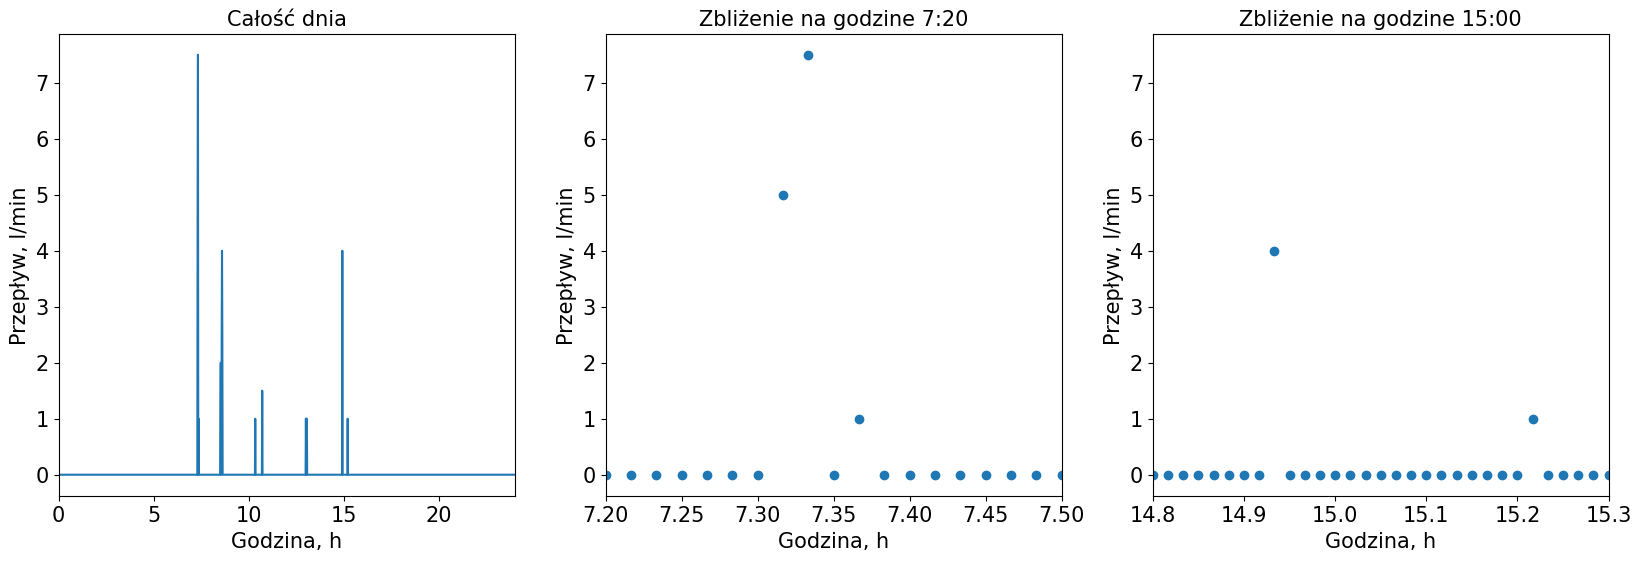
\includegraphics[width=1\textwidth]{img/Dane_nowe_disp.png}
	\caption{Podpis rysunku zawsze pod rysunkiem.}
	\label{fig:etykieta-rysunku}
\end{figure}\\
Pierwszy wykres przestawia dane zebrane z domu nr. 13 zebrane w dniu 05/02/2018. Oś X oznaczająca godzinę, począwszy od północy. Oś Y reprezentuje przepływ wody w danym momencie dnia. Wykres Przestwia nieregularne piki o nierównomiernym rozkładzie. Okresami o zwiększonym przepływie są godziny 7-13 oraz 14-15. Okresy mniejszej aktywyności możemy zaobserwowac w godzinach późno popołudniowych oraz nocnych. Drugi i trzeci wykres przedstawiają zbiżenie na godzine 7 oraz 15. Dzięki zwężeniu analizowanego zakresu czasu, możliwe było dokładniejsze zbadanie struktury występujących pików. Ta metoda wizualizacji ujawniła, że poszczególne piki, które na ogólnym wykresie dobowym mogły sprawiać wrażenie pojedynczych punktów, w rzeczywistości są złożone z wielu pojedynczych zdarzeń. To odkrycie jest istotne, ponieważ wskazuje na bardziej złożoną dynamikę przepływu w określonych momentach doby, co na pierwszy rzut oka mogło umknąć uwadze.\\
\newpage
W celu lepszego wstępnego zrozumienia charakterystyki analizowanego zestawu danych, niezbędne jest także szczegółowe przyjrzenie się kilku losowo wybranym domostwom.\\
\begin{figure}[!h]
	\centering
	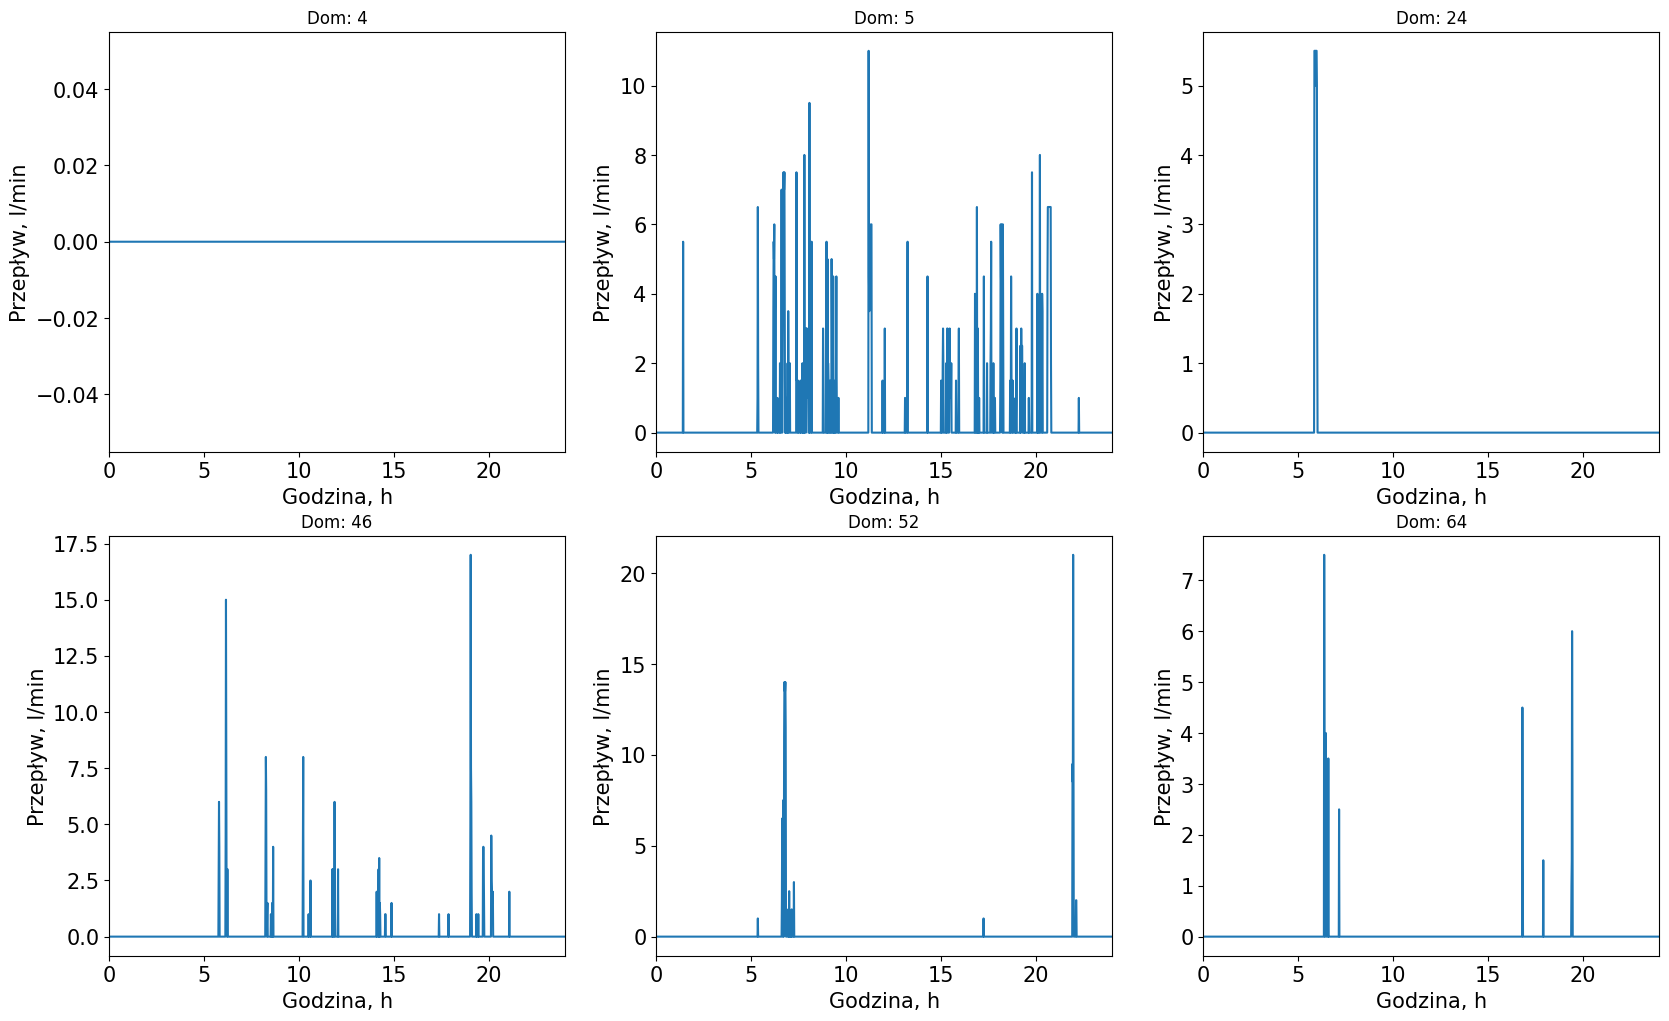
\includegraphics[width=1\textwidth]{img/Dane_nowe_compare.png}
	\caption{Porównanie przepływów dla przykładowych domów w dniu 05/02/2018}
	\label{fig:etykieta-rysunku}
\end{figure}\\
Analiza przedstawionych histogramów przepływów dla poszczególnych losowo wybranych domostw, wykonana na podstawie danych z dnia 05/02/2018, ukazuje wyraźne różnice w charakterystyce przepływów dla każdego z nich. Zgodnie z Rysunkiem 3.2, można stwierdzić, że każdy dom prezentuje unikalny wzór aktywności, co może odzwierciedlać różnorodność nawyków, planów dnia lub specyficznych potrzeb mieszkańców. Na przykład, dla domu nr 5 zużycie wody jest rozłożone przez większą część dnia, z obserwowaną aktywnością w rozmaitych godzinach. Jednakże, zarejestrowano również pojedyncze zużycie w nocy. Z kolei Dom 52 charakteryzuje się wyraźnym szczytem wieczornym, co stanowi kontrast w stosunku do pozostałych domów.\\W przypadku Domu nr 4, nie odnotowano żadnego przepływu w analizowanym dniu. Brak danych może wynikać z co najmniej dwóch potencjalnych przyczyn. Pierwszą z nich jest zastosowany czas próbkowania, który wynosił jedną minutę. Taki interwał może nie być wystarczająco krótki, aby zarejestrować sporadyczne lub krótkotrwałe zdarzenia przepływu. Drugą możliwością, która może wyjaśniać brak zarejestrowanej aktywności, jest potencjalna nieobecność mieszkańców w domu w danym dniu.

\newpage
Pomimo iż zgromadzone dane charakteryzowały się wysoką jakością, ich specyficzny format wymagał przygotowania skryptu celem ich przetwarzania i ekstrakcję istotnych informacji.\\
\begin{figure}[!h]
	\centering
	\lstinputlisting[language=Python]{kod/Przetwarzanie_nowe_dane.py}
	\caption{Fragment skryptu przetwarzającego dane.}
	\label{fig:pseudokod:listings}
\end{figure}

W ramach procesu dostowania formatu aby przystosować go do wymagań tensorflow, dzień tygodnia zostal zamieniona na etykiete liczbową, która przyjmuje wartośc od 1 do 7, co odpowiada kolejnym dniom tygodnia. Podobny proces został zastosowany do etykietowania pór roku. Każda została zakodowana jako etykieta w zakresie od 1 do 4 co prezentuje kolejno, wiosne, lato, jesień i zimę. Dodatkowo czas dnia został zmieniony na procent dnia w skali od 0 do 1.
\section{Projektowanie i ocena modeli}
W ramach realizacji badań nad optymalizacją architektury sieci neuronowej oraz doborem hiperparametrów, zdecydowano się na podział danych uczących na trzy zbiory. Pierwszy z nich to zestaw który zawiera dane pochodzące z 12 losowo wybranych domostw, co ma na celu zapewnienie reprezentatywności i różnorodności w ramach próby badawczej. Drugi zestaw stanowi podzbiór zawierający dane z pojedynczego gospodarstwa domowego, co pozwala na szczegółową analizę wydajności modelu w warunkach bardziej jednorodnych danych. Dodatkowo, utworzony został trzeci zestaw danych, który obejmował informacje z wszystkich 77 domów biorących udział w badaniu.


Podział zbioru danych na trzy zestawy okazał się kluczowy dla efektywnego doboru hiperparametrów modelu, szczególnie biorąc pod uwagę, że cały zbiór danych zawierał aż 12,5 miliona wierszy. Zestaw wybranych domostw, zawierający blisko 2 miliony wierszy, oraz pojedyncze domostwo z 161 tysiącami wierszy, umożliwiły przeprowadzenie dokładniejszych i bardziej zróżnicowanych testów.

Czas uczenia sieci był znacząco różny dla poszczególnych zestawów danych. Przykładowo, dla całego zbioru danych proces uczenia trwający 10 epok przy rozmiarze partii równym 64 zajmował około 46 minut. Tymczasem dla wybranych domostw czas ten skracał się do 9 minut, a dla pojedynczego domostwa uczenie trwało zaledwie 40 sekund. W ramach badań podjęto próby wykorzystania Google Colab, będącego popularnym narzędziem służącym do programowania i przetwarzania danych w chmurze. Po odpowiednim skonfigurowaniu środowiska, napotkano na pierwszy znaczący problem - czas trwania uploadu pliku. Zaskakująco, przesyłanie pliku o rozmiarze 300 MB, zawierającego 12,5 miliona wierszy, zajęło znacznie więcej czasu, niż można było przewidywać. Kolejnym krokiem było przeprowadzenie procesu uczenia maszynowego na danych, zaplanowanego na 10 epok. Niestety, cały proces trwał ponad 100 minut, co wskazuje na ograniczenia wersji darmowej Google Colab. W związku z tym, stwierdzono, że bez inwestycji w wersję płatną, Google Colab nie zapewnia oczekiwanej redukcji czasu niezbędnego do nauki modelu

Początkowo hiperparametry były testowane na najmniejszym zbiorze, co pozwalało na szybką i efektywną ocenę różnych konfiguracji. Po uzyskaniu zadowalających wyników na zbiorze pojedynczego domostwa, testy były rozszerzane kolejno na zbiór wybranych domostw, a następnie na pełny zbiór danych. Taka strategia pozwoliła na stopniowe i metodyczne dostosowywanie hiperparametrów, minimalizując przy tym czas i zasoby potrzebne do przeprowadzenia eksperymentów, a jednocześnie maksymalizując ogólną skuteczność modelu.
\begin{table}[!h]
	\centering
	\caption{Hiperparametry Sieci Neuronowej}
	\begin{tabular}{|c|c|c|c|}
		\hline
		Optymalizator & Funkcja strat & Początkowy współczynnik uczenia & Rozmiar partii \\ \hline
		Adam          & mse           & 0.0001                          & 64             \\ \hline
	\end{tabular}
\end{table}

Po przeprowadzeniu serii eksperymentów, w procesie selekcji optymalnej architektury sieci neuronowej, najbardziej efektywną konfiguracją okazała się struktura składająca się z sześciu warstw, z których cztery pełniły funkcję warstw ukrytych. W procesie iteracyjnego dostosowywania i ewaluacji różnych architektur sieci, model o takiej budowie wykazał najlepsze wyniki w zakresie dokładności i generalizacji na testowanych zbiorach danych. Architektura ta charakteryzowała się kolejno malejącą liczbą neuronów w poszczególnych warstwach: pierwsza warstwa zawierała 512 neuronów, druga 256, trzecia 128, czwarta 64, piąta 32, a szósta, będąca warstwą wyjściową, miała 1 neuron. Wszystkie warstwy, z wyjątkiem ostatniej, wykorzystywały funkcję aktywacji ReLU. Natomiast ostatnia warstwa, pełniąca rolę warstwy wyjściowej, zastosowała funkcję aktywacji typu 'linear'


W ramach opracowanego modelu sieci neuronowej zastosowano dynamicznie zmieniający się współczynnik uczenia, oparty na metodzie wykładniczego spadku, opisanego wzorem:
\begin{equation}
	\text{Wspołczynik uczenia}(epoka) =
	\begin{cases}
		\text{Początkowy wspołczynik uczenia}                 & \text{jeżeli } epoka < 5    \\
		\text{Wspołczynik uczenia}(epoka - 1) \times e^{-0.1} & \text{jeżeli } epoka \geq 5
	\end{cases}
\end{equation}
Użycie tej motyody pozwoliło na zmniejszanie wartości współczynnika uczenia w trakcie procesu trenowania, co zwiększyło zdolności adaptacyjne sieci. Został on zastosowany gdyż częstym zjawiskiem było generowanie przez sieć stałej wartości wyjściowej, niezależnie od różnych danych wejściowych.

W ramach procesu testowania różnych konfiguracji sieci neuronowej zaproponowano eksplorację wydajności modeli przy różnorodnych kombinacjach wejść. Celem tego podejścia było zbadanie, jak zmiana danych wejściowych wpłynie na zdolność modelu do nauki i generalizacji przewidywania przepływu. Poniżej przedstawiono zestawienie modeli, które zostały uwzględnione w analizie:

\begin{enumerate}
	\item Model A
	      \begin{enumerate}
		      \item Wejścia: Dzień tygodnia, pora dnia
		      \item Wyjście: Przepływ
	      \end{enumerate}
	\item Model B
	      \begin{enumerate}
		      \item Wejścia: pora dnia
		      \item Wyjście: Przepływ
	      \end{enumerate}
	\item Model C
	      \begin{enumerate}
		      \item Wejścia: pora roku, dzień tygodnia, pora dnia
		      \item Wyjście: Przepływ
	      \end{enumerate}
	\item Model D
	      \begin{enumerate}
		      \item Wejścia: pora roku, pora dnia
		      \item Wyjście: Przepływ
	      \end{enumerate}
\end{enumerate}

Wyniki te dostarczą wglądu w to, które wejścia są najbardziej wartościowe dla modelowania przepływu oraz czy dodanie dodatkowych informacji kontekstowych przyczynia się do znaczącej poprawy wyników predykcyjnych.
\newpage

\section{Walidacja i próby dostrajania (?)}
W celu weryfikacji poprawności i efektywności opracowanego modelu sieci neuronowej, przeprowadzono porównanie modelu nauczonych na danych ze wszystkich 12 domostw z modelami utworzonymi dla każdego z tych domów osobno. Taki eksperyment miał na celu ocenę zdolności generalizacji modelu nauczonych na zbiorze 12 domostw w porównaniu z modelami specyficznymi dla poszczególnych domów.

\begin{figure}[!h]
	\centering
	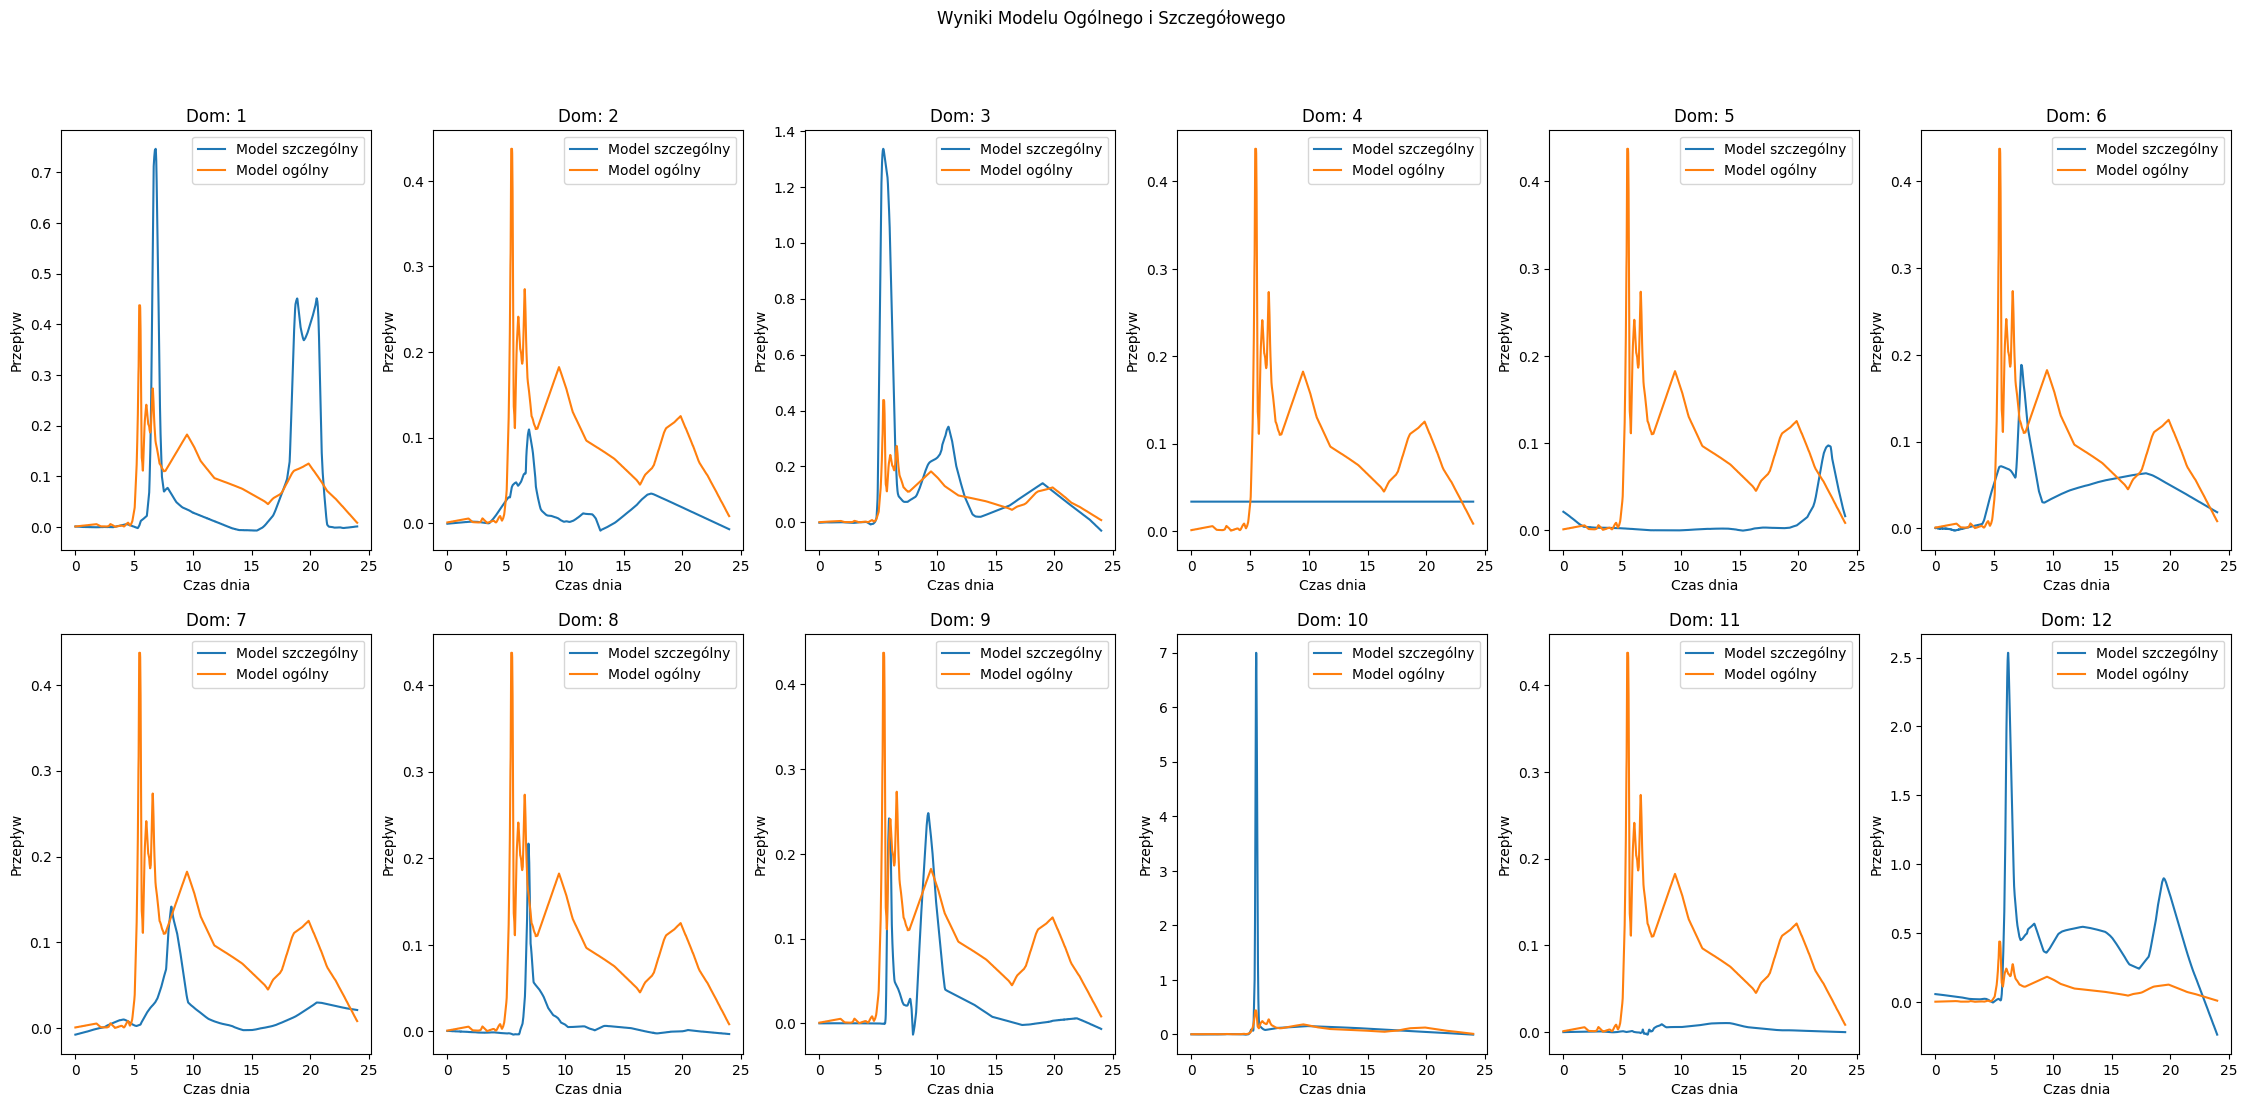
\includegraphics[width=1\textwidth]{img/szczegółowy_ogolny_porówniaie.png}
	\caption{Porównianie modelu ogólnego z modelami szczególnymi}
	\label{fig:etykieta-rysunku}
\end{figure}

W celu dalszego zwiększenia skuteczności modelu sieci neuronowej zaproponowano wprowadzenie dodatkowego wejścia do systemu – tygodniowego zużycia. Implementacja tego rozwiązania została przeprowadzona w specyficzny sposób, mający na celu uniknięcie przekształcenia tego parametru w niezamierzony label identyfikujący poszczególne domy. W fazie uczenia modelu, do każdego tygodnia przypisywano sumę zużycia zarejestrowanego w tym okresie. Natomiast w fazie testowania, model otrzymywał średnią wartość tygodniowego zużycia. Celem tej strategii było umożliwienie modelowi korzystania z danych historycznych zużycia w sposób, który poprawiałby jego zdolność do przewidywania, jednocześnie zachowując elastyczność i możliwość generalizacji wyników na różne domostwa.

\newpage

\begin{figure}[!h]
	\centering
	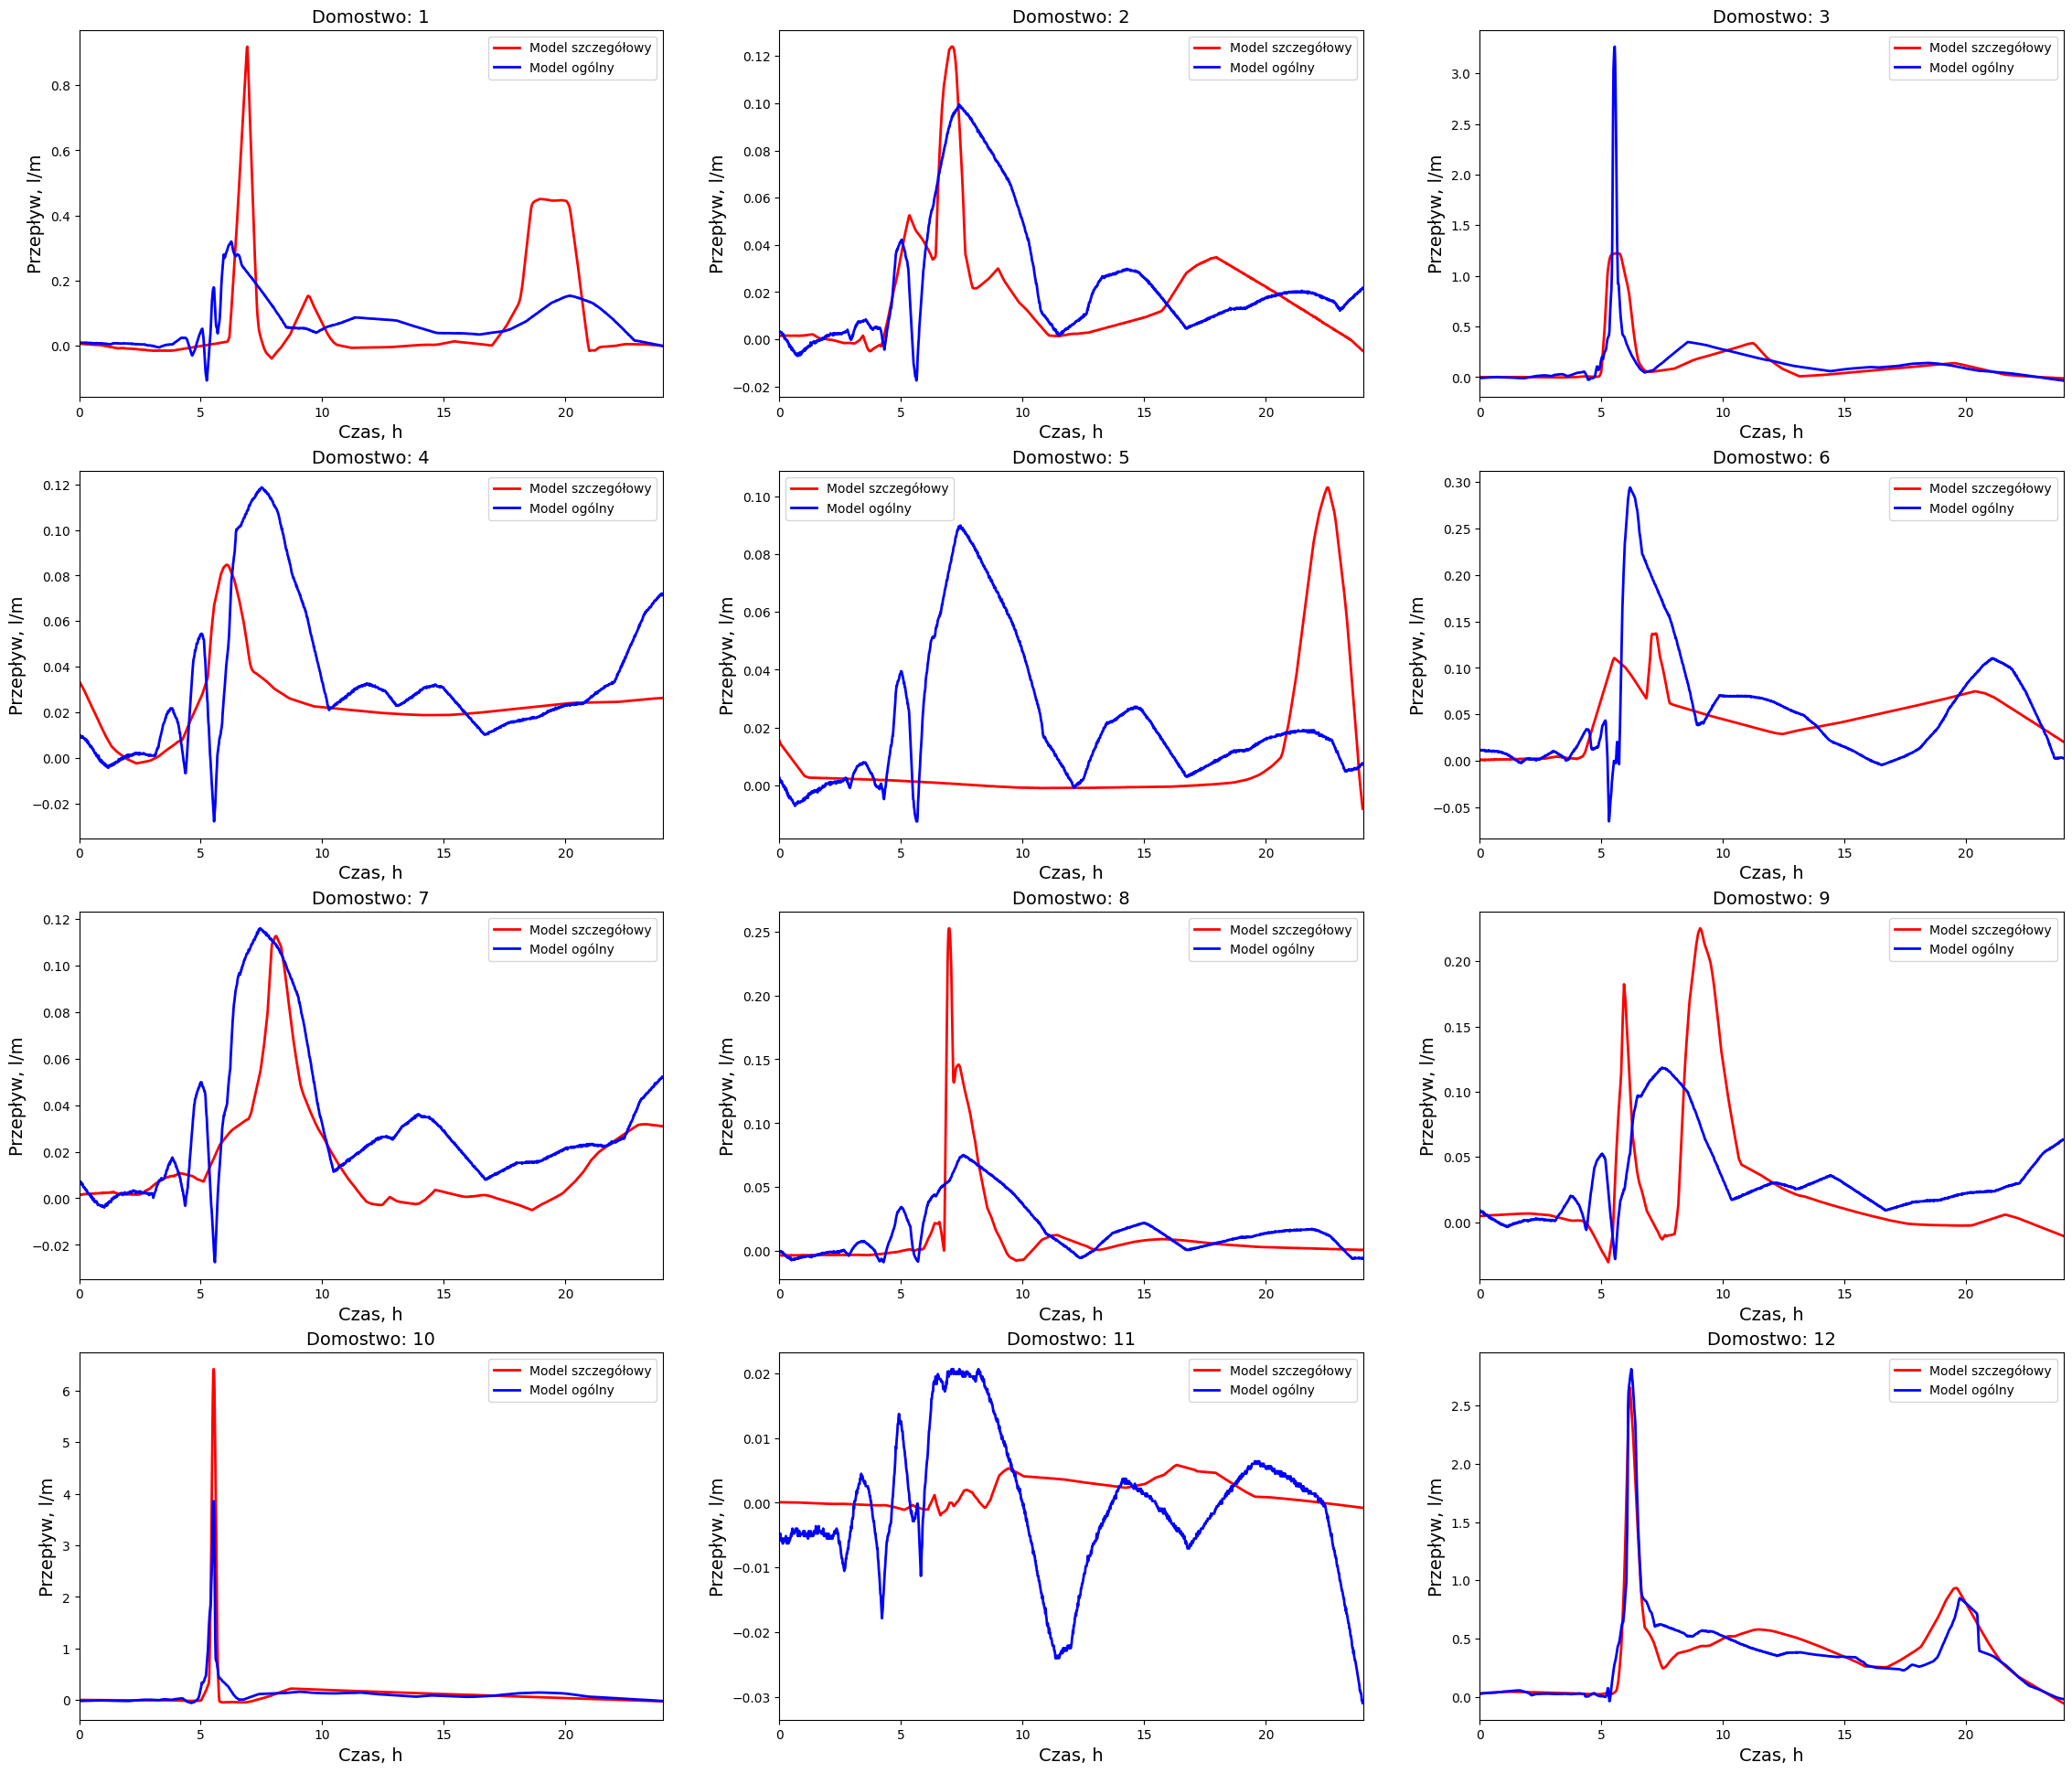
\includegraphics[width=1\textwidth]{img/szczegółowy_ogolny_porówniaie_dodatkowy.png}
	\caption{Porównianie modelu ogólnego z modelami szczególnymi po dodaniu kolejnego wejścia do sieci}
	\label{fig:etykieta-rysunku}
\end{figure}

Analizując charakterystykę modelu ogólnego i szczególnego dla każdego z domostw, przedstawioną na Rysunku 3.5, można zauważyć, że dla domostwa nr 10 i 12 model ogólny wykazał się wysoką zgodnością z modelem szczegółowym, co świadczy o jego zdolności do precyzyjnego odwzorowania charakterystyki przewidywania przepływu w ciągu dnia. W przypadku tych dwóch domów, przebieg przewidywań dla obu modeli jest podobny, co wskazuje na to, że model ogólny efektywnie uchwycił dynamikę zużycia charakterystyczną dla tych konkretnych domostw. Natomiast w kontekście Domu nr 5, wyniki ukazują, że model ogólny miał znaczne trudności z dopasowaniem się do wzorców przepływu.

W celu dokładniejszej oceny i porównania efektywności modelu ogólnego, nauczonego na danych z 12 domostw, z modelami szczegółowymi, nauczonymi dla poszczególnych domów, zastosowano wskaźnik błędu średniokwadratowego. MSE, obliczany jako średnia kwadratów różnic między wartościami przewidywanymi przez model a rzeczywistymi danymi, posłużył jako miara odchylenia modelu ogólnego od wyników modeli szczegółowych. W tym kontekście, niższa wartość MSE wskazywała na lepszą zgodność modelu ogólnego z wynikami modeli szczegółowych, sugerując, że model ogólny skuteczniej generalizuje dane, zbliżając się do precyzji modeli trenowanych na danych z pojedynczych domostw.

\begin{table}[!h]
	\centering
	\caption{Porównianie wartości MSE dla każdego obu modelów}
	\resizebox{\textwidth}{!}{
		\begin{tabular}{|c|cccccccccccc|}
			\hline
			\multirow{2}{*}{MSE} & \multicolumn{12}{c|}{DOMOSTWO}                                                                                                                                                                                                                                                                                                                        \\ \cline{2-13}
			                     & \multicolumn{1}{c|}{1}         & \multicolumn{1}{c|}{2}       & \multicolumn{1}{c|}{3}     & \multicolumn{1}{c|}{4}       & \multicolumn{1}{c|}{5}      & \multicolumn{1}{c|}{6}      & \multicolumn{1}{c|}{7}       & \multicolumn{1}{c|}{8}       & \multicolumn{1}{c|}{9}      & \multicolumn{1}{c|}{10}    & \multicolumn{1}{c|}{11}      & 12    \\ \hline
			Model 1              & \multicolumn{1}{c|}{0.022}     & \multicolumn{1}{c|}{0.0074}  & \multicolumn{1}{c|}{0.037} & \multicolumn{1}{c|}{0.0067}  & \multicolumn{1}{c|}{0.011}  & \multicolumn{1}{c|}{0.0039} & \multicolumn{1}{c|}{0.0084}  & \multicolumn{1}{c|}{0.0095}  & \multicolumn{1}{c|}{0.0072} & \multicolumn{1}{c|}{0.22}  & \multicolumn{1}{c|}{0.010}   & 0.19  \\ \hline
			Model 2              & \multicolumn{1}{c|}{0.019}     & \multicolumn{1}{c|}{0.00053} & \multicolumn{1}{c|}{0.034} & \multicolumn{1}{c|}{0.00085} & \multicolumn{1}{c|}{0.0013} & \multicolumn{1}{c|}{0.0025} & \multicolumn{1}{c|}{0.00055} & \multicolumn{1}{c|}{0.00069} & \multicolumn{1}{c|}{0.0027} & \multicolumn{1}{c|}{0.075} & \multicolumn{1}{c|}{0.00013} & 0.019 \\ \hline
		\end{tabular}
	}
\end{table}

Analizując przedstawione dane w tabeli, można zauważyć, że po dodaniu dodatkowego wejścia do systemu, czyli tygodniowego zużycia, model 2 (Model z dodatkowym wejściem) osiągnął znacznie lepsze wyniki w porównaniu z modelem bazowym. Wartości błędu średniokwadratowego dla modelu 2 są niższe w porównaniu do modelu 1 dla każdego z domostw, co wskazuje na poprawę dokładności predykcji.
Na przykład, dla Domu nr 2, MSE zmniejszyło się z 0.0074 w modelu 1 do 0.00053 w modelu 2, co jest znaczącą poprawą. Podobne znaczące redukcje można zaobserwować w przypadku Domu nr 12, gdzie MSE spadło z 0.19 do 0.019


\chapter{Pogoda}
\label{ch:0X}

\begin{figure}[!h]
	\centering
	\includegraphics[width=1\textwidth]{img/Pogoda_porównanie.png}
	\caption{Porównanie warunkuch atmosferycznych na przestrzeni dnia}
	\label{fig:etykieta-rysunku}
\end{figure}
W celu zbadania wpływu wielkości modelu na wyniki oraz sprawdzenia ważności różnych wejść, zaproponowano w badaniu dwa modele o różnej złożoności architektury. Oba modele korzystały z tej samej funkcji harmonogramowania tempa uczenia, która redukowała szybkość uczenia po czwartej epoce, oraz z tych samych parametrów kompilacji, w tym optymalizatora Adam z początkową szybkością uczenia 0.001, funkcji straty MSE
Pierwszy model składał się z mniejszej liczby warstw i neuronów: warstwa normalizująca, trzy warstwy gęste z odpowiednio 64, 32 i 1 neuronami, używając funkcji aktywacji 'relu' dla pierwszych dwóch warstw i 'linear' dla warstwy wyjściowej.
Drugi model był znacznie większy, zawierając więcej warstw i neuronów: warstwa normalizująca, sześć warstw gęstych o zwiększającej się liczbie neuronów: 1024, 512, 256, 128, 64, 32, zakończonych warstwą wyjściową z 1 neuronem, używając funkcji aktywacji 'relu' dla warstw ukrytych i 'linear' dla warstwy wyjściowej.
Oba modele były trenowane przez 50 epok z rozmiarem partii równym 32. Celem porównania tych dwóch modeli było ustalenie, czy zwiększenie liczby warstw i neuronów w modelu wpłynie na jego

W ramach procesu weryfikacji skuteczności zastosowanych modeli sieci neuronowych, dane zostały podzielone w proporcji 80\% do 20\%. Ta strategia podziału danych miała na celu zapewnienie solidnej bazy do nauki modeli oraz efektywnej oceny ich wydajności. Model numer 1 wykazał się niższą skutecznością w porównaniu do modelu numer 2. Świadczy o tym wartość błędu średniokwadratowego, która dla modelu pierwszego wyniosła 0.0668, natomiast dla modelu drugiego było to znacząco niższe, a mianowicie 0.0237. Ta różnica w wartościach MSE wskazuje na wyższą precyzję i efektywność modelu numer 2 w procesie uczenia i oceny na podstawie dostępnych danych.
\section{Permutacyjna Ważność Cech}
Permutacyjna Ważność Cech, to technika stosowana w uczeniu maszynowym do oceny znaczenia poszczególnych wejść dla modelu predykcyjnego. Metoda ta jest stosowana zarówno dla modeli klasyfikacyjnych, jak i regresyjnych. Proces ten rozpoczyna się od trenowania modelu na oryginalnym zestawie danych, co pozwala na ustalenie bazowej wydajności modelu. Następnie przeprowadza się permutację każdej cechy z osobna w zbiorze testowym, losowo mieszając jej wartości, podczas gdy wszystkie inne cechy pozostają niezmienione. Po dokonaniu permutacji, model jest ponownie oceniany na zmodyfikowanym zbiorze danych. Wyniki tej oceny są następnie porównywane z wynikami uzyskanymi na oryginalnym, niezmodyfikowanym zbiorze. Różnica w wydajności modelu, taka jak spadek dokładności w klasyfikacji lub wzrost błędu średniokwadratowego w regresji, jest wykorzystywana do oceny ważności danej cechy. Im większy spadek wydajności, tym większa uważana jest ważność tej cechy dla modelu.

W kontekście wykorzystania PFI do oceny ważności cech w modelu, istotne jest zwrócenie uwagi na kwestię korelacji między danymi. PFI opiera się na permutacji pojedynczych cech, co oznacza zmianę wartości jednej zmiennej niezależnie od pozostałych. W przypadku, gdy dane są silnie skorelowane, taka metoda permutacji może prowadzić do błędnych wniosków

W celu implementacji techniki PFI w pracy, został wykorzystany obiekt PermutationImportance z biblioteki sklearn. Zastosowanie tego dedykowanego narzędzia umożliwiło nie tylko dokładną, ale i wydajną realizację tej metody, co pozwoliło na jej skuteczną integrację z procesem badawczym.

\begin{table}[!h]
	\centering
	\caption{Porównianie wartości MSE dla każdego obu modelów}
	\resizebox{\textwidth}{!}{
		\begin{tabular}{|c|c|c|c|c|c|c|}
			\hline
			             & \begin{tabular}[c]{@{}c@{}}Temperatura \\ zewnętrzna\end{tabular} & \begin{tabular}[c]{@{}c@{}}Wilgotność\\  zewnętrzna\end{tabular} & \begin{tabular}[c]{@{}c@{}}Ciśnienie\\  atmosferyczne\end{tabular} & \begin{tabular}[c]{@{}c@{}}Prędkość\\  wiatru\end{tabular} & \begin{tabular}[c]{@{}c@{}}Kierunek\\  wiatru\end{tabular} & \begin{tabular}[c]{@{}c@{}}Wilgotność \\ wewnętrzna\end{tabular} \\ \hline
			Model krótki & 0.57                                                              & 0.45                                                             & 1.00                                                               & 0.50                                                       & 0.17                                                       & 0.60                                                             \\ \hline
			Model długi  & 0.47                                                              & 0.11                                                             & 0.65                                                               & 0.23                                                       & 0.17                                                       & 1.00                                                             \\ \hline
		\end{tabular}
	}
\end{table}

\newpage
\section{Badanie wag wejściowych pierwszej warsty}
W analizie modeli uczenia maszynowego, interpretacja wag pierwszej warstwy może służyć jako metoda określania ważności cech wejściowych. Ponieważ wagi w pierwszej warstwie sieci neuronowej są bezpośrednio połączone z cechami wejściowymi, wartości tych wag mogą dostarczać informacji o znaczeniu poszczególnych cech dla predykcji modelu. Wysoka wartość wagowa sugeruje, że zmiana wartości tej cechy wejściowej może mieć istotny wpływ na wynik modelu. Jednakże, ta metoda interpretacji może być mniej efektywna w przypadku bardziej złożonych, głębokich sieci neuronowych. W takich modelach, liczne warstwy i skomplikowane struktury, w tym nieliniowe aktywacje i interakcje między neuronami, mogą skutkować tym, że bezpośredni wpływ pojedynczych wag jest trudniejszy do zrozumienia.
\begin{figure}[!h]
	\centering
	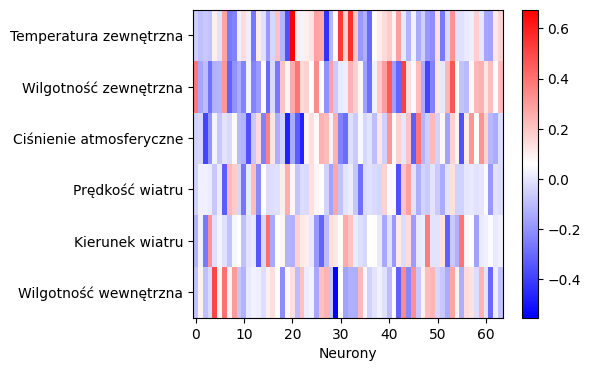
\includegraphics[width=0.7\textwidth]{img/heatmap1.png}
	\caption{Mapa ciepła wag pierwszej warstwy dla modelu o uproszczonej architekturze}
	\label{fig:etykieta-rysunku}
\end{figure}

Mapa ciepła wag pierwszej warstwy sieci neuronowej stanowi cenne narzędzie analityczne, pozwalające na wizualną interpretację i zrozumienie wpływu dużej liczby cech na proces uczenia. Jest to instrument szczególnie użyteczny w kontekście wysokowymiarowych zbiorów danych, gdzie tradycyjne metody analizy mogą okazać się niewystarczające. W przedstawionym przypadku, analiza mapy ciepła nie ujawnia istotnych anomalii w rozkładzie wag. Obserwuje się jedynie sporadyczne wartości, które odstają od średnich wag, lecz nie osiągają one poziomu znacząco wpływającego na wyniki modelu.

W celu dokładnej analizy ważności poszczególnych wag wejściowych sieci neuronowej przeprowadzono obliczenie średniej wartości wagi dla każdego z wejść. Procedura ta umożliwiła identyfikację względnej ważności cech poprzez porównanie ich przeciętnego wpływu na aktywację neuronów w modelu. Następnie, aby umożliwić porównywalność wyników niezależnie od ich pierwotnej skali, dokonano normalizacji obliczonych średnich wag.
\begin{table}[!h]
	\centering
	\caption{Todo}
	\resizebox{\textwidth}{!}{
		\begin{tabular}{|c|c|c|c|c|c|}
			\hline
			\begin{tabular}[c]{@{}c@{}}Temperatura \\ zewnętrzna\end{tabular} & \begin{tabular}[c]{@{}c@{}}Wilgotność\\  zewnętrzna\end{tabular} & \begin{tabular}[c]{@{}c@{}}Ciśnienie\\  atmosferyczne\end{tabular} & \begin{tabular}[c]{@{}c@{}}Prędkość\\  wiatru\end{tabular} & \begin{tabular}[c]{@{}c@{}}Kierunek\\  wiatru\end{tabular} & \begin{tabular}[c]{@{}c@{}}Wilgotność \\ wewnętrzna\end{tabular} \\ \hline
			0.57                                                              & 0.45                                                             & 1.00                                                               & 0.50                                                       & 0.17                                                       & 0.60                                                             \\ \hline
		\end{tabular}
	}
\end{table}

Analizy bardziej złożonych modeli sieci neuronowych, metoda interpretacji wag pierwszej warstwy może okazać się nieefektywna. Ze względu na zwiększoną głębokość i złożoność architektury, wagi w pierwszej warstwie tracą bezpośrednią i jednoznaczną interpretowalność, która jest charakterystyczna dla prostszych modeli. W modelach rozbudowanych, cechy wejściowe przechodzą przez wiele warstw transformacji, co skutkuje utratą bezpośredniego powiązania między wagami pierwszej warstwy a wynikowymi decyzjami modelu. W efekcie, interpretacja tych wag może nie odzwierciedlać faktycznego wpływu poszczególnych cech na decyzje modelu, co jest spowodowane nakładaniem się, transformacją i połączeniem informacji w kolejnych warstwach sieci.

\begin{figure}[!h]
	\centering
	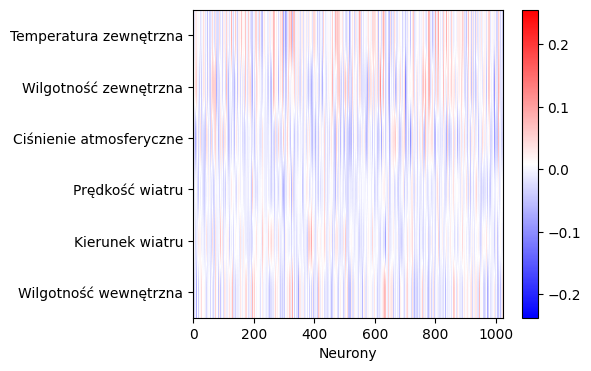
\includegraphics[width=0.7\textwidth]{img/heatmap2.png}
	\caption{Mapa ciepła wag pierwszej warstwy dla modelu o rozbudowanej architekturze}
	\label{fig:etykieta-rysunku}
\end{figure}

\begin{table}[!h]
	\centering
	\caption{Todo}
	\resizebox{\textwidth}{!}{
		\begin{tabular}{|c|c|c|c|c|c|}
			\hline
			\begin{tabular}[c]{@{}c@{}}Temperatura \\ zewnętrzna\end{tabular} & \begin{tabular}[c]{@{}c@{}}Wilgotność\\  zewnętrzna\end{tabular} & \begin{tabular}[c]{@{}c@{}}Ciśnienie\\  atmosferyczne\end{tabular} & \begin{tabular}[c]{@{}c@{}}Prędkość\\  wiatru\end{tabular} & \begin{tabular}[c]{@{}c@{}}Kierunek\\  wiatru\end{tabular} & \begin{tabular}[c]{@{}c@{}}Wilgotność \\ wewnętrzna\end{tabular} \\ \hline
			1.00                                                              & 0.11                                                             & 0.75                                                               & 0.73                                                       & 0.61                                                       & 0.13                                                             \\ \hline
		\end{tabular}
	}
\end{table}

\newpage
\section{LIME}
W kontekście zrozumienia modeli uczenia maszynowego, metoda Local Interpretable Model-agnostic Explanations jest istotnym narzędziem, które umożliwia interpretację decyzji modelu na poziomie lokalnym. Metoda ta wyróżnia się spośród innych, takich jak SHAP, dzięki swojemu unikalnemu podejściu skoncentrowanemu na pojedynczych instancjach danych. Podczas gdy SHAP dąży do zapewnienia ogólnego zrozumienia wpływu cech na model przez zbieranie i analizowanie informacji z różnych instancji, LIME skupia się na wyjaśnieniu, w jaki sposób model dokonuje przewidywań dla konkretnej, wybranej próbki danych.

Podstawowym elementem metody LIME jest modyfikacja danych i tworzenie na ich podstawie uproszczonego modelu, który ma za zadanie odwzorować zachowanie oryginalnego, skomplikowanego modelu, ale tylko w ograniczonym, lokalnym obszarze wokół analizowanej instancji. Proces ten rozpoczyna się od stworzenia zbioru danych przez modyfikację wybranej instancji, co skutkuje powstaniem podobnych, ale nieidentycznych przykładów. Następnie, na tych zmodyfikowanych danych, oblicza się przewidywania za pomocą oryginalnego modelu. Kluczowym krokiem jest trenowanie prostego modelu, takiego jak regresja liniowa, na podstawie tych przewidywań. Model ten służy do aproksymacji wpływu zmian w danych na przewidywania modelu. W ten sposób, analizując współczynniki modelu liniowego, można zrozumieć, które cechy miały największy wpływ na przewidywania dla danej instancji.

W ramach pracy, w celu dokładnej oceny skuteczności metody LIME, zdecydowano się na zastosowanie jej na losowo wybranych próbkach ze zbioru testowego.

\begin{table}[!h]
	\caption{Todo}
	\resizebox{\textwidth}{!}{
		\begin{tabular}{|c|c|c|c|c|c|}
			\hline
			\begin{tabular}[c]{@{}c@{}}Temperatura \\ zewnętrzna\end{tabular} & \begin{tabular}[c]{@{}c@{}}Wilgotność\\  zewnętrzna\end{tabular} & \begin{tabular}[c]{@{}c@{}}Ciśnienie\\  atmosferyczne\end{tabular} & \begin{tabular}[c]{@{}c@{}}Prędkość\\  wiatru\end{tabular} & \begin{tabular}[c]{@{}c@{}}Kierunek\\  wiatru\end{tabular} & \begin{tabular}[c]{@{}c@{}}Wilgotność \\ wewnętrzna\end{tabular} \\ \hline
			0.17                                                              & 0.57                                                             & 1.00                                                               & 0.09                                                       & 0.00                                                       & 0.00                                                             \\ \hline
			1.00                                                              & 0.36                                                             & 0.08                                                               & 0.04                                                       & 0.02                                                       & 0.36                                                             \\ \hline
			1.00                                                              & 0.02                                                             & 0.02                                                               & 0.04                                                       & 0.00                                                       & 0.32                                                             \\ \hline
			0.13                                                              & 1.00                                                             & 0.53                                                               & 0.00                                                       & 0.00                                                       & 0.47                                                             \\ \hline
		\end{tabular}
	}
\end{table}

Mimo iż LIME jest metodą zasadniczo skoncentrowaną na dostarczaniu interpretacji lokalnych, istnieje możliwość adaptacji jej do generowania wniosków o charakterze bardziej ogólnym. Można to osiągnąć poprzez zastosowanie metody LIME wielokrotnie na różnych próbkach danych, a nastepnie wyciąganięcie średniej. Zaproponowano wybranie czterech zestawów ze zbioru testowego, zawierających odpowiednio 10, 50, 100, i 1000 próbek.


\begin{table}[!h]
	\caption{Todo}
	\resizebox{\textwidth}{!}{
		\begin{tabular}{|c|c|c|c|c|c|c|}
			\hline
			\begin{tabular}[c]{@{}c@{}}Ilość\\ próbek\end{tabular} & \begin{tabular}[c]{@{}c@{}}Temperatura \\ zewnętrzna\end{tabular} & \begin{tabular}[c]{@{}c@{}}Wilgotność\\  zewnętrzna\end{tabular} & \begin{tabular}[c]{@{}c@{}}Ciśnienie\\  atmosferyczne\end{tabular} & \begin{tabular}[c]{@{}c@{}}Prędkość\\  wiatru\end{tabular} & \begin{tabular}[c]{@{}c@{}}Kierunek\\  wiatru\end{tabular} & \begin{tabular}[c]{@{}c@{}}Wilgotność\\  wewnętrzna\end{tabular} \\ \hline
			10                                                     & 0.95                                                              & 0.82                                                             & 1.00                                                               & 0.20                                                       & 0.21                                                       & 0.09                                                             \\ \hline
			50                                                     & 1.00                                                              & 0.21                                                             & 0.53                                                               & 0.15                                                       & 0.03                                                       & 0.01                                                             \\ \hline
			100                                                    & 1.00                                                              & 0.27                                                             & 0.53                                                               & 0.26                                                       & 0.05                                                       & 0.02                                                             \\ \hline
			1000                                                   & 1.00                                                              & 0.41                                                             & 0.49                                                               & 0.15                                                       & 0.01                                                       & 0.01                                                             \\ \hline
		\end{tabular}
	}
\end{table}


\chapter{Modelowanie zbiornika CWU}
\label{ch:05}
\section{Metodologia}
\subsection{Opis matematyczny modelu}
\begin{equation}
	\frac{dT_{wo}^{3}}{dt} = b_1^3 F_z (T_{zi} - T_{wo}^{3}) - b_2^3 F_w (T_{wo}^{3} - T_{wo}^{2}) - b_3^4 (T_{wo}^{3} - T_{ot})
\end{equation}

\begin{equation}
	\frac{dT_{zi}}{dt} = p_1 Q_g - p_2 F_z (T_{zi} - T_{wo}^{3}) - p_3 (T_{zi} - T_{ot})
\end{equation}

\begin{equation}
	\frac{dT_{wo}^{2}}{dt} = b_1^2 F_z (T_{zi} - T_{wo}^{2}) - b_2^2 F_w (T_{wo}^{2} - T_{wo}^{1}) - b_3^2 (T_{wo}^{2} - T_{ot}) - b_4^2 (T_{wo}^{2} - T_{wo}^{1}) + b_5^2 (T_{wo}^{3} - T_{wo}^{2})
\end{equation}

\begin{equation}
	\frac{dT_{wo}^{1}}{dt} = -b_2^1 F_w (T_{wo}^{1} - T_{wi}) - b_3^1 (T_{wo}^{1} - T_{ot}) + b_5^1 (T_{wo}^{2} - T_{wo}^{1})
\end{equation}

Przedstawienie modelu warstwowego, równań stanu, pokazanie wyników symulacji modelu
\section{Wyniki symulacji}


% Jeśli „Specyfikacja wewnętrzna”:
% \begin{itemize}
% 	\item przedstawienie idei
% 	\item architektura systemu
% 	\item opis struktur danych (i organizacji baz danych)
% 	\item komponenty, moduły, biblioteki, przegląd ważniejszych klas (jeśli występują)
% 	\item przegląd ważniejszych algorytmów (jeśli występują)
% 	\item szczegóły implementacji wybranych fragmentów, zastosowane wzorce projektowe
% 	\item diagramy UML
% \end{itemize}

% % % % % % % % % % % % % % % % % % % % % % % % % % % % % % % % % % % 
% Pakiet minted wymaga importu: \usepackage{minted}                 %
% i specjalnego kompilowania:                                       %
% pdflatex -shell-escape main                                       %
% % % % % % % % % % % % % % % % % % % % % % % % % % % % % % % % % % % 


Krótka wstawka kodu w linii tekstu jest możliwa, np.  \lstinline|int a;| (biblioteka \texttt{listings})% lub  \mintinline{C++}|int a;| (biblioteka \texttt{minted})
.
Dłuższe fragmenty lepiej jest umieszczać jako rysunek, np. kod na rys \ref{fig:pseudokod:listings}% i rys. \ref{fig:pseudokod:minted}
, a naprawdę długie fragmenty – w załączniku.

%\begin{figure}
%\centering
%\begin{minted}[linenos,frame=lines]{c++}
%class test : public basic
%{
%    public:
%      test (int a);
%      friend std::ostream operator<<(std::ostream & s, 
%                                     const test & t);
%    protected:
%      int _a;  
%      
%};
%\end{minted}
%\caption{Pseudokod w \texttt{minted}.}
%\label{fig:pseudokod:minted}
%\end{figure}


\chapter{Optymalizacja}
\label{ch:06}
\section{Funkcja kosztów}
\begin{equation}
	G = \int p_1 Q_g \, dt
\end{equation}
\section{Funkcja komfortu}
\begin{equation}
	J = \int \left( T_{wo} - T_{wym} \right)^2 \left| \frac{\text{sign}(T_{wo} - T_{wym} - \delta) + \text{sign}(T_{wo} - T_{wym} + \delta)}{2} \right| \, dt
\end{equation}


\begin{itemize}
	\item sposób testowania w ramach pracy (np. odniesienie do modelu V)
	\item organizacja eksperymentów
	\item przypadki testowe zakres testowania (pełny/niepełny)
	\item wykryte i usunięte błędy
	\item opcjonalnie wyniki badań eksperymentalnych
\end{itemize}

\begin{table}
	\centering
	\caption{Nagłówek tabeli jest nad tabelą.}
	\label{id:tab:wyniki}
	\begin{tabular}{rrrrrrrr}
		\toprule
		        & \multicolumn{7}{c}{metoda}                                                                                                                                  \\
		\cmidrule{2-8}
		        &                            &         & \multicolumn{3}{c}{alg. 3} & \multicolumn{2}{c}{alg. 4, $\gamma = 2$}                                                \\
		\cmidrule(r){4-6}\cmidrule(r){7-8}
		$\zeta$ & alg. 1                     & alg. 2  & $\alpha= 1.5$              & $\alpha= 2$                              & $\alpha= 3$ & $\beta = 0.1$ & $\beta = -0.1$ \\
		\midrule
		0       & 8.3250                     & 1.45305 & 7.5791                     & 14.8517                                  & 20.0028     & 1.16396       & 1.1365         \\
		5       & 0.6111                     & 2.27126 & 6.9952                     & 13.8560                                  & 18.6064     & 1.18659       & 1.1630         \\
		10      & 11.6126                    & 2.69218 & 6.2520                     & 12.5202                                  & 16.8278     & 1.23180       & 1.2045         \\
		15      & 0.5665                     & 2.95046 & 5.7753                     & 11.4588                                  & 15.4837     & 1.25131       & 1.2614         \\
		20      & 15.8728                    & 3.07225 & 5.3071                     & 10.3935                                  & 13.8738     & 1.25307       & 1.2217         \\
		25      & 0.9791                     & 3.19034 & 5.4575                     & 9.9533                                   & 13.0721     & 1.27104       & 1.2640         \\
		30      & 2.0228                     & 3.27474 & 5.7461                     & 9.7164                                   & 12.2637     & 1.33404       & 1.3209         \\
		35      & 13.4210                    & 3.36086 & 6.6735                     & 10.0442                                  & 12.0270     & 1.35385       & 1.3059         \\
		40      & 13.2226                    & 3.36420 & 7.7248                     & 10.4495                                  & 12.0379     & 1.34919       & 1.2768         \\
		45      & 12.8445                    & 3.47436 & 8.5539                     & 10.8552                                  & 12.2773     & 1.42303       & 1.4362         \\
		50      & 12.9245                    & 3.58228 & 9.2702                     & 11.2183                                  & 12.3990     & 1.40922       & 1.3724         \\
		\bottomrule
	\end{tabular}
\end{table}



% TODO
\chapter{Podsumowanie i wnioski}
\begin{itemize}
	\item uzyskane wyniki w świetle postawionych celów i zdefiniowanych wyżej wymagań
	\item kierunki ewentualnych danych prac (rozbudowa funkcjonalna …)
	\item problemy napotkane w trakcie pracy
\end{itemize}



\backmatter

%\bibliographystyle{plplain}  % bibtex
%\bibliography{biblio} % bibtex
\printbibliography           % biblatex
\addcontentsline{toc}{chapter}{Bibliografia}

\begin{appendices}

	% TODO
	\chapter{Spis skrótów i symboli}

	\begin{itemize}
		\item[$T_{zi}^{?}$]
		\item[$T_{wo}^{?}$]
		\item[$T_{ot}$]
		\item[$Q_p$]
		\item[$F_w$]
		\item[$F_z$]
		\item[n] numer warstwy
		\item[m] numer źródła ciepła
	\end{itemize}


	% TODO
	\chapter{Źródła}

	Jeżeli w pracy konieczne jest umieszczenie długich fragmentów kodu źródłowego, należy je przenieść w to miejsce.

	\begin{lstlisting}
if (_nClusters < 1)
	throw std::string ("unknown number of clusters");
if (_nIterations < 1 and _epsilon < 0)
	throw std::string ("You should set a maximal number of iteration or minimal difference -- epsilon.");
if (_nIterations > 0 and _epsilon > 0)
	throw std::string ("Both number of iterations and minimal epsilon set -- you should set either number of iterations or minimal epsilon.");
\end{lstlisting}


	% % % % % % % % % % % % % % % % % % % % % % % % % % % % % % % % % % % 
	% Pakiet minted wymaga odkomentowania w pliku config/settings.tex   %
	% importu pakietu minted: \usepackage{minted}                       %
	% i specjalnego kompilowania:                                       %
	% pdflatex -shell-escape praca                                      %
	% % % % % % % % % % % % % % % % % % % % % % % % % % % % % % % % % % % 

	%\begin{minted}[linenos,breaklines,frame=lines]{c++}
	%if (_nClusters < 1)
	%   throw std::string ("unknown number of clusters");
	%if (_nIterations < 1 and _epsilon < 0)
	%   throw std::string ("You should set a maximal number of iteration or minimal difference -- epsilon.");
	%if (_nIterations > 0 and _epsilon > 0)
	%   throw std::string ("Both number of iterations and minimal epsilon set -- you should set either number of iterations or minimal epsilon.");
	%\end{minted}


	% TODO
	\chapter{Lista dodatkowych plików, uzupełniających tekst pracy}


	W systemie do pracy dołączono dodatkowe pliki zawierające:
	\begin{itemize}
		\item źródła programu,
		\item dane testowe,
		\item film pokazujący działanie opracowanego oprogramowania lub zaprojektowanego i~wykonanego urządzenia,
		\item itp.
	\end{itemize}


	\listoffigures
	\addcontentsline{toc}{chapter}{Spis rysunków}
	\listoftables
	\addcontentsline{toc}{chapter}{Spis tabel}

\end{appendices}

\end{document}


%% Finis coronat opus.

